%
% teil3.tex -- Eigenschaften der Bessel-Funktionen
%
% (c) 2026 Gian Cavegn, OST Ostschweizer Fachhochschule
%
% !TEX root = ../../buch.tex
% !TEX encoding = UTF-8
% !TeX spellcheck = de_CH
%
\section{Eigenschaften der Bessel-Funktionen
\label{bessel:section:eigenschaften}}
\kopfrechts{Eigenschaften}
%
% Dieser Abschnitt ist der Werkzeugkasten. Alles, was hier steht, wird
% später gebraucht.
%   - Rekursionsformeln       -> Rechnen allgemein
%   - Integraldarstellung     -> teil6 (Kepler), das ist die Brücke!
%   - Nullstellen             -> Membran
%   - Orthogonalität          -> Fourier-Bessel-Reihe, Membran
%   - Asymptotik              -> Vergleich mit cos
%
Die Reihe~\eqref{bessel:loesung:eqn:jnu} definiert die Bessel-Funktionen, ist zum Rechnen aber unhandlich.
Dieser Abschnitt stellt die Eigenschaften zusammen, mit denen man tatsächlich arbeitet.
Es lohnt sich, dabei immer den Vergleich mit den trigonometrischen Funktionen im Auge zu behalten.
Fast jede Eigenschaft von $J_\nu$ hat ein Gegenstück bei $\cos$ und $\sin$.

%
% Rekursionsformeln
%
\subsection{Rekursionsformeln
\label{bessel:eigenschaften:subsection:rekursion}}
Aus der Reihendarstellung lassen sich zwei Ableitungsformeln direkt ablesen.

\begin{satz}
\label{bessel:eigenschaften:satz:ableitung}
Für alle $\nu$ gilt
\begin{align}
\frac{d}{dx}
\bigl( x^{\nu} J_\nu(x) \bigr)
&=
x^{\nu} J_{\nu-1}(x),
\label{bessel:eigenschaften:eqn:ableitung1}
\\
\frac{d}{dx}
\bigl( x^{-\nu} J_\nu(x) \bigr)
&=
-x^{-\nu} J_{\nu+1}(x).
\label{bessel:eigenschaften:eqn:ableitung2}
\end{align}
\end{satz}
 
\begin{proof}
Aus~\eqref{bessel:loesung:eqn:jnu} folgt
\[
x^\nu J_\nu(x)
=
\sum_{k=0}^\infty
\frac{(-1)^k}{k!\,\Gamma(\nu+k+1)}
\frac{x^{2k+2\nu}}{2^{2k+\nu}}.
\]
Gliedweises Differenzieren ist innerhalb des Konvergenzbereiches erlaubt und ergibt
\[
\frac{d}{dx}
\bigl( x^\nu J_\nu(x) \bigr)
=
\sum_{k=0}^\infty
\frac{(-1)^k (2k+2\nu)}{k!\,\Gamma(\nu+k+1)}
\frac{x^{2k+2\nu-1}}{2^{2k+\nu}}.
\]
Wegen $1/\Gamma(z)=z/\Gamma(z+1)$, das ist die Funktionalgleichung~\eqref{bessel:loesung:eqn:gammafunktional} für die ganze Funktion $1/\Gamma$, gilt
\[
\frac{2k+2\nu}{\Gamma(\nu+k+1)}
=
\frac{2}{\Gamma(\nu+k)}
\]
auch dann, wenn $\nu+k$ eine nichtpositive ganze Zahl ist.
Damit bleibt genau die Reihe von $x^\nu J_{\nu-1}(x)$.
Die zweite Formel folgt analog.
\end{proof}
 
Führt man die Produktregel aus und eliminiert einmal die Ableitung und einmal $J_\nu$, erhält man die beiden für die Praxis wichtigsten Beziehungen.
 
\begin{korollar}
\label{bessel:eigenschaften:korollar:rekursion}
Es gilt
\begin{align}
J_{\nu-1}(x) + J_{\nu+1}(x)
&=
\frac{2\nu}{x} J_\nu(x),
\label{bessel:eigenschaften:eqn:dreiterm}
\\
J_{\nu-1}(x) - J_{\nu+1}(x)
&=
2 J_\nu'(x).
\label{bessel:eigenschaften:eqn:ableitungrek}
\end{align}
\end{korollar}
 
Die erste Formel ist eine Dreitermrekursion.
\index{Dreitermrekursion}%
Kennt man $J_0$ und $J_1$, so lassen sich alle weiteren Ordnungen daraus berechnen.
Aus~\eqref{bessel:eigenschaften:eqn:ableitungrek} folgt für $\nu=0$ wegen $J_{-1}=-J_1$ der oft gebrauchte Spezialfall
\begin{equation}
J_0'(x) = -J_1(x),
\label{bessel:eigenschaften:eqn:j0strich}
\end{equation}
das genaue Gegenstück zu $\cos' = -\sin$.
 
%
% Erzeugende Funktion und Integraldarstellung
%
\subsection{Erzeugende Funktion und Integraldarstellung
\label{bessel:eigenschaften:subsection:erzeugend}}
Für ganzzahlige Ordnungen gibt es eine überraschend kompakte Beschreibung aller $J_n$ auf einmal.
\index{erzeugende Funktion}%
 
\begin{satz}
\label{bessel:eigenschaften:satz:erzeugend}
Für $t\ne 0$ gilt
\begin{equation}
e^{\frac{x}{2}\left(t-\frac{1}{t}\right)}
=
\sum_{n=-\infty}^{\infty}
J_n(x)\, t^n.
\label{bessel:eigenschaften:eqn:erzeugend}
\end{equation}
\end{satz}
 
\begin{proof}
Beide Faktoren lassen sich in ihre Exponentialreihe entwickeln,
\[
e^{\frac{x}{2}t}
=
\sum_{p=0}^\infty
\frac{1}{p!}
\biggl(\frac{x}{2}\biggr)^{p} t^{p},
\qquad
e^{-\frac{x}{2t}}
=
\sum_{q=0}^\infty
\frac{(-1)^q}{q!}
\biggl(\frac{x}{2}\biggr)^{q} t^{-q}.
\]
Für $t\ne 0$ konvergieren beide Reihen absolut, das Produkt darf deshalb ausmultipliziert und beliebig umgeordnet werden,
\[
e^{\frac{x}{2}\left(t-\frac{1}{t}\right)}
=
\sum_{p=0}^\infty
\sum_{q=0}^\infty
\frac{(-1)^q}{p!\,q!}
\biggl(\frac{x}{2}\biggr)^{p+q}
t^{p-q}.
\]
Den Koeffizienten von $t^n$ erhält man, indem man alle Paare $(p,q)$ mit $p-q=n$ zusammenfasst.
Für $n\ge 0$ sind das die Paare $p=n+k$ und $q=k$ mit $k\ge 0$, und wegen $p+q=2k+n$ ist der Koeffizient
\[
\sum_{k=0}^\infty
\frac{(-1)^k}{(n+k)!\,k!}
\biggl(\frac{x}{2}\biggr)^{2k+n}
=
J_n(x)
\]
nach~\eqref{bessel:loesung:eqn:jnu}.
Für $n=-m$ mit $m>0$ kommt die Bedingung $p\ge 0$ hinzu, die Summation beginnt also erst bei $k=m$.
Die Substitution $k=m+j$ liefert
\[
\sum_{j=0}^\infty
\frac{(-1)^{m+j}}{j!\,(m+j)!}
\biggl(\frac{x}{2}\biggr)^{2j+m}
=
(-1)^m J_m(x)
=
J_{-m}(x),
\]
wobei im letzten Schritt das in Abschnitt~\ref{bessel:loesung:subsection:ynu} bewiesene Verhalten von $J_{-n}$ verwendet wurde.
\end{proof}
 
Setzt man $t=e^{i\tau}$, so wird $t-1/t = 2i\sin\tau$, und \eqref{bessel:eigenschaften:eqn:erzeugend} geht über in
\begin{equation}
e^{ix\sin\tau}
=
\sum_{n=-\infty}^{\infty}
J_n(x)\, e^{in\tau}.
\label{bessel:eigenschaften:eqn:jacobianger}
\end{equation}
Das ist die \emph{Jacobi-Anger-Entwicklung}.
\index{Jacobi-Anger-Entwicklung}%
Die rechte Seite ist eine Fourier-Reihe in $\tau$, und die $J_n(x)$ sind ihre Fourier-Koeffizienten.
Die übliche Formel für Fourier-Koeffizienten liefert damit sofort das folgende Korollar.

\begin{korollar}
\label{bessel:eigenschaften:korollar:integral}
Für $n\in\mathbb{Z}$ gilt
\begin{equation}
J_n(x)
=
\frac{1}{2\pi}
\int_{-\pi}^{\pi}
e^{i(x\sin\tau - n\tau)}\,d\tau
=
\frac{1}{\pi}
\int_0^{\pi}
\cos(n\tau - x\sin\tau)\,d\tau.
\label{bessel:eigenschaften:eqn:integral}
\end{equation}
\end{korollar}
 
Diese Integraldarstellung ist historisch die ursprüngliche.
\index{Integraldarstellung, Bessel-Funktion}%
\index{Bessel-Funktion!Integraldarstellung}%
Bessel hat die Funktionen in dieser Form eingeführt, und sie ist die Brücke zur Kepler-Gleichung in Abschnitt~\ref{bessel:section:kepler}.
Für $n=1$ ist der Ausdruck $\tau - x\sin\tau$ im Integranden bereits die linke Seite der Kepler-Gleichung.

Die Jacobi-Anger-Entwicklung hat ausserdem eine geometrische Bedeutung, die den Bogen zurück zu Abschnitt~\ref{bessel:herleitung:subsection:polar} schlägt.
Mit $x=kr$ und $\tau=\varphi$ ist die linke Seite von~\eqref{bessel:eigenschaften:eqn:jacobianger} gleich $e^{ikr\sin\varphi}=e^{iky}$, also eine ebene Welle, die in $y$-Richtung läuft.
Die Glieder der rechten Seite sind die Produkte $J_n(kr)e^{in\varphi}$, und das sind genau die separierten Lösungen $R(r)\Phi(\varphi)$ der Helmholtz-Gleichung aus der Herleitung.
Die Entwicklung sagt also, wie eine ebene Welle in Polarkoordinaten aussieht, nämlich als Überlagerung der separierten Lösungen mit den Bessel-Funktionen als Amplituden.

%
% Nullstellen
%
\subsection{Nullstellen
\label{bessel:eigenschaften:subsection:nullstellen}}
Die Bessel-Funktionen oszillieren, und ihre Nullstellen bestimmen in jeder Anwendung die möglichen Eigenfrequenzen.
\index{Bessel-Funktion!Nullstellen}%
\index{Eigenfrequenz}%
Warum sie oszillieren, sieht man an einer kleinen Umformung der Bessel-Gleichung.
Ist $y$ eine Lösung von~\eqref{bessel:loesung:eqn:bessel}, zum Beispiel $y=J_\nu$, und schreibt man $y(x)=x^{-1/2}u(x)$, so fällt beim Einsetzen der Term mit der ersten Ableitung weg, und für $u$ bleibt
\begin{equation}
u''
+
\Bigl(
1
+
\frac{\frac14-\nu^2}{x^2}
\Bigr)
u
=
0.
\label{bessel:eigenschaften:eqn:normalform}
\end{equation}
Der Faktor $x^{-1/2}$ ändert nichts an den Nullstellen, $u$ und $J_\nu$ verschwinden für $x>0$ an denselben Stellen.
Für grosse $x$ ist der Bruch in~\eqref{bessel:eigenschaften:eqn:normalform} vernachlässigbar, und übrig bleibt die Schwingungsgleichung $u''+u=0$ mit den Lösungen $\cos$ und $\sin$.
Weit draussen verhält sich $J_\nu$ also wie eine Schwingung mit Nullstellen im Abstand $\pi$, und Abbildung~\ref{bessel:loesung:fig:jnu} zeigt genau das.
Nahe bei $0$ stört der Bruch, deshalb liegen die ersten Nullstellen noch nicht im Abstand $\pi$.

\begin{satz}
\label{bessel:eigenschaften:satz:nullstellen}
Für $\nu\ge 0$ hat $J_\nu$ unendlich viele positive Nullstellen
\[
0 < j_{\nu,1} < j_{\nu,2} < j_{\nu,3} < \dots,
\]
und zwischen zwei aufeinanderfolgenden Nullstellen von $J_\nu$ liegt genau eine Nullstelle von $J_{\nu+1}$.
\end{satz}

Der erste Teil ist die präzise Form der eben beschriebenen Beobachtung.
Sein Beweis vergleicht~\eqref{bessel:eigenschaften:eqn:normalform} mit der Schwingungsgleichung und findet sich bei \cite[Kapitel~XV]{bessel:watson}, eine Übersicht über die Nullstellen gibt \cite[Abschnitt~10.21]{bessel:dlmf}.
Der zweite Teil steckt in der Ableitungsformel~\eqref{bessel:eigenschaften:eqn:ableitung2}.
\index{Satz!von Rolle}%
Die Funktion $x^{-\nu}J_\nu(x)$ verschwindet an zwei aufeinanderfolgenden Nullstellen von $J_\nu$, nach dem Satz von Rolle verschwindet ihre Ableitung dazwischen, und diese Ableitung ist bis auf den Faktor $-x^{-\nu}$ gerade $J_{\nu+1}$.
Dasselbe Argument mit~\eqref{bessel:eigenschaften:eqn:ableitung1} und der Funktion $x^{\nu+1}J_{\nu+1}(x)$ liefert eine Nullstelle von $J_\nu$ zwischen zwei Nullstellen von $J_{\nu+1}$.
Die Nullstellen der beiden Funktionen wechseln sich also ab, und in Abbildung~\ref{bessel:loesung:fig:jnu} kann man das an $J_0$ und $J_1$ nachprüfen.

Die Nullstellen sind nicht in geschlossener Form angebbar, sie müssen numerisch bestimmt werden.
Tabelle~\ref{bessel:eigenschaften:tab:nullstellen} zeigt die ersten Werte.

\begin{table}
\centering
\caption{Die ersten vier positiven Nullstellen $j_{\nu,m}$ der Bessel-Funktionen $J_\nu$ für ganzzahlige Ordnung, gerundet auf vier Nachkommastellen.
Die Werte sind \cite[Abschnitt~9.5]{bessel:abramowitz} entnommen.
\label{bessel:eigenschaften:tab:nullstellen}}
\begin{tabular}{c|cccc}
$\nu$ & $j_{\nu,1}$ & $j_{\nu,2}$ & $j_{\nu,3}$ & $j_{\nu,4}$ \\
\hline
$0$ & $2.4048$ & $5.5201$ & $8.6537$ & $11.7915$ \\
$1$ & $3.8317$ & $7.0156$ & $10.1735$ & $13.3237$ \\
$2$ & $5.1356$ & $8.4172$ & $11.6198$ & $14.7960$ \\
$3$ & $6.3802$ & $9.7610$ & $13.0152$ & $16.2235$
\end{tabular}
\end{table}
 
Anders als bei $\sin$ sind die Nullstellen nicht äquidistant, ihre Abstände nähern sich aber für grosse $x$ dem Wert $\pi$ an.
Das ist die Erklärung für den unharmonischen Klang einer Trommel.
Die Eigenfrequenzen der kreisförmigen Membran vom Radius $a$ ergeben sich aus der Randbedingung $R(a)=0$ für die Lösung $R(r)=J_n(kr)$ von~\eqref{bessel:herleitung:eqn:radial}, also aus $J_n(ka)=0$, zu
\begin{equation}
\omega_{nm}
=
\frac{c}{a}\, j_{n,m}.
\label{bessel:eigenschaften:eqn:eigenfrequenzen}
\end{equation}
Das Verhältnis der beiden tiefsten rotationssymmetrischen Moden ist $j_{0,2}/j_{0,1}\approx 2.295$ und damit kein ganzzahliges Vielfaches des Grundtons.
Bei der Saite dagegen liegen die Nullstellen des Sinus äquidistant, und die Obertöne sind ganzzahlige Vielfache der Grundfrequenz.
Abbildung~\ref{bessel:eigenschaften:fig:moden} zeigt die vier tiefsten Moden mit ihren Knotenlinien.

\begin{figure}
\centering
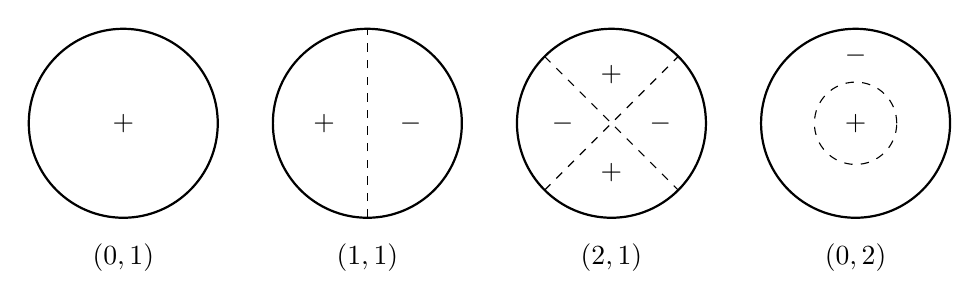
\begin{tikzpicture}
% Mode (0,1)
\begin{scope}
	\draw[thick] (0,0) circle (1.2);
	\node at (0,0) {$+$};
	\node at (0,-1.7) {$(0,1)$};
\end{scope}
% Mode (1,1)
\begin{scope}[xshift=3.1cm]
	\draw[thick] (0,0) circle (1.2);
	\draw[dashed] (0,-1.2) -- (0,1.2);
	\node at (-0.55,0) {$+$};
	\node at (0.55,0) {$-$};
	\node at (0,-1.7) {$(1,1)$};
\end{scope}
% Mode (2,1)
\begin{scope}[xshift=6.2cm]
	\draw[thick] (0,0) circle (1.2);
	\draw[dashed] (-0.849,-0.849) -- (0.849,0.849);
	\draw[dashed] (-0.849,0.849) -- (0.849,-0.849);
	\node at (0,0.62) {$+$};
	\node at (0,-0.62) {$+$};
	\node at (-0.62,0) {$-$};
	\node at (0.62,0) {$-$};
	\node at (0,-1.7) {$(2,1)$};
\end{scope}
% Mode (0,2)
\begin{scope}[xshift=9.3cm]
	\draw[thick] (0,0) circle (1.2);
	\draw[dashed] (0,0) circle (0.523);
	\node at (0,0) {$+$};
	\node at (0,0.86) {$-$};
	\node at (0,-1.7) {$(0,2)$};
\end{scope}
\end{tikzpicture}
\caption{Die vier tiefsten Schwingungsmoden der kreisförmigen Membran.
Der erste Index $n$ zählt die Knotendurchmesser und stammt aus dem Winkelanteil $\cos n\varphi$, der zweite Index $m$ nummeriert die Nullstelle $j_{n,m}$ und bestimmt die Zahl der Knotenkreise im Innern.
Die gestrichelten Linien sind die Knotenlinien, die Vorzeichen geben die Phase der Auslenkung an.
Der innere Knotenkreis der Mode $(0,2)$ liegt bei $j_{0,1}/j_{0,2}\approx 0.436$ des Radius.
Die Frequenzen verhalten sich nach \eqref{bessel:eigenschaften:eqn:eigenfrequenzen} wie $1 : 1.593 : 2.136 : 2.295$.
\label{bessel:eigenschaften:fig:moden}}
\end{figure}
 
%
% Orthogonalität
%
\subsection{Orthogonalität
\label{bessel:eigenschaften:subsection:orthogonalitaet}}
Die Sinusfunktionen $\sin m\pi s$ sind auf $[0,1]$ orthogonal, darauf beruht die Fourier-Reihe der Saite.
\index{Orthogonalitat@Orthogonalität}%
\index{Bessel-Funktion!Orthogonalitat@Orthogonalität}%
\index{Fourier-Reihe}%
Für die Bessel-Funktionen gilt dasselbe, wenn man als Variable den auf den Membranradius bezogenen Radius $s=r/a$ nimmt, die Nullstellen $j_{\nu,m}$ als Skalierung verwendet und das Integral mit dem Gewicht $s$ versieht.
\index{Gewichtsfunktion}%

\begin{satz}
\label{bessel:eigenschaften:satz:orthogonalitaet}
Sind $j_{\nu,m}$ und $j_{\nu,l}$ positive Nullstellen von $J_\nu$, so gilt
\begin{equation}
\int_0^1
J_\nu(j_{\nu,m}s)\,
J_\nu(j_{\nu,l}s)\,
s\,ds
=
\begin{cases}
0 & \text{für } m\ne l,\\[3pt]
\dfrac{1}{2}\,J_{\nu+1}(j_{\nu,m})^2 & \text{für } m=l.
\end{cases}
\label{bessel:eigenschaften:eqn:orthogonalitaet}
\end{equation}
\end{satz}

Der Grund für die Orthogonalität ist derselbe wie bei den Eigenvektoren einer symmetrischen Matrix.
Die Funktionen $J_\nu(j_{\nu,m}s)$ sind die Radialanteile der Eigenschwingungen der Membran aus Abschnitt~\ref{bessel:eigenschaften:subsection:nullstellen}, und Eigenschwingungen zu verschiedenen Frequenzen stehen senkrecht aufeinander.
Der Beweis schreibt die Bessel-Gleichung für beide Funktionen hin, multipliziert über Kreuz, subtrahiert und integriert, die Randterme fallen wegen $J_\nu(j_{\nu,m})=0$ weg.
Er findet sich zusammen mit der Rechnung für den Fall $m=l$ bei \cite[S.~132--136]{bessel:watson} und in \cite[Formel~10.22.37]{bessel:dlmf}.

Die Bedeutung der Orthogonalität ist dieselbe wie bei jeder Orthogonalbasis.
Eine Funktion lässt sich eindeutig als Linearkombination der Basisfunktionen darstellen, und die Koeffizienten erhält man durch Skalarprodukte mit den Basisfunktionen, wobei das Skalarprodukt hier das Integral mit dem Gewicht $s$ ist.
Eine auf $[0,1]$ hinreichend gutartige Funktion $f$ lässt sich als
\begin{equation}
f(s)
=
\sum_{m=1}^{\infty}
c_m J_\nu(j_{\nu,m}s)
\label{bessel:eigenschaften:eqn:fourierbessel}
\end{equation}
entwickeln, mit den Koeffizienten
\begin{equation}
c_m
=
\frac{2}{J_{\nu+1}(j_{\nu,m})^2}
\int_0^1 f(s)\,J_\nu(j_{\nu,m}s)\,s\,ds.
\label{bessel:eigenschaften:eqn:fourierkoeffizienten}
\end{equation}
Das ist die \emph{Fourier-Bessel-Reihe}.
\index{Fourier-Bessel-Reihe}%
Die Formel für $c_m$ erhält man, indem man die Reihe mit $J_\nu(j_{\nu,m}s)\,s$ multipliziert und über $[0,1]$ integriert, denn nach Satz~\ref{bessel:eigenschaften:satz:orthogonalitaet} bleibt von der Summe nur ein Glied übrig.
Für welche Funktionen die Reihe konvergiert, ist eine eigene Frage, die bei \cite[Kapitel~XVIII]{bessel:watson} und in \cite[Abschnitt~10.23]{bessel:dlmf} beantwortet wird.

Für die Membran heisst das, dass sich jede rotationssymmetrische Anfangsauslenkung $f(r/a)$ eindeutig in die Eigenschwingungen $J_0(j_{0,m}r/a)$ zerlegen lässt, genau wie eine Fourier-Reihe die Anfangsauslenkung einer Saite in ihre Obertöne zerlegt.
Das Gewicht $s$ ist dabei kein Schönheitsfehler, sondern das Flächenelement der Polarkoordinaten, denn mit $s=r/a$ ist $dA=r\,dr\,d\varphi=a^2s\,ds\,d\varphi$.
Das Integral mit dem Gewicht $s$ ist also das Integral über die Kreisscheibe, und die Orthogonalität der Bessel-Funktionen ist die natürliche Orthogonalität auf der Scheibe.

%
% Asymptotisches Verhalten
%
\subsection{Asymptotisches Verhalten
\label{bessel:eigenschaften:subsection:asymptotik}}
Für grosse Argumente werden die Bessel-Funktionen fast zu trigonometrischen Funktionen.
\index{asymptotisches Verhalten}%
\index{Bessel-Funktion!Asymptotik}%

\begin{satz}
\label{bessel:eigenschaften:satz:asymptotik}
Für $x\to\infty$ gilt
\begin{equation}
J_\nu(x)
=
\sqrt{\frac{2}{\pi x}}
\cos\Bigl(x-\frac{\nu\pi}{2}-\frac{\pi}{4}\Bigr)
+
O(x^{-3/2}).
\label{bessel:eigenschaften:eqn:asymptotikj}
\end{equation}
\end{satz}

Die Gestalt dieser Formel erklärt sich aus der Normalform~\eqref{bessel:eigenschaften:eqn:normalform} in Abschnitt~\ref{bessel:eigenschaften:subsection:nullstellen}.
Für grosse $x$ bleibt von ihr die Schwingungsgleichung $u''+u=0$ übrig, $u$ ist also asymptotisch eine Schwingung mit Kreisfrequenz eins, und der Faktor $1/\sqrt{x}$ kommt von der Rücksubstitution $J_\nu=x^{-1/2}u$.
Die Amplitude $\sqrt{2/\pi}$ und die Phase $-\nu\pi/2-\pi/4$ liefert dieses Argument nicht, sie erfordern eine genauere Analyse, die bei \cite[Kapitel~VII]{bessel:watson} und in \cite[Formel~10.17.3]{bessel:dlmf} nachzulesen ist.
Ein Sonderfall lässt sich aber direkt nachrechnen.
Für $\nu=\frac12$ verschwindet der Bruch in~\eqref{bessel:eigenschaften:eqn:normalform}, die Normalform ist dann exakt die Schwingungsgleichung, und tatsächlich gilt
\begin{equation}
J_{1/2}(x)
=
\sqrt{\frac{2}{\pi x}}\,\sin x ,
\label{bessel:eigenschaften:eqn:jhalb}
\end{equation}
wie man durch Einsetzen von $\nu=\frac12$ in die Reihe~\eqref{bessel:loesung:eqn:jnu} bestätigt.
Das stimmt mit~\eqref{bessel:eigenschaften:eqn:asymptotikj} überein, denn für $\nu=\frac12$ ist das Phasenargument $x-\frac{\pi}{2}$, und es gilt $\cos(x-\frac{\pi}{2})=\sin x$.
Die zweite Lösung $Y_\nu$ aus Abschnitt~\ref{bessel:loesung:subsection:ynu} hat dieselbe Asymptotik mit $\sin$ anstelle von $\cos$.

Die Abklingrate $1/\sqrt{x}$ ist physikalisch einleuchtend.
Eine von einem Punkt ausgehende Kreiswelle verteilt ihre Energie auf einen Kreis mit Umfang $2\pi r$, die Energiedichte fällt also wie $1/r$ und die Amplitude wie $1/\sqrt{r}$.
Wirft man einen Stein ins Wasser, sieht man genau das.

Zusammen mit~\eqref{bessel:loesung:eqn:kleinx} ist das Verhalten von $J_\nu$ damit in beiden Grenzfällen bekannt.
Nahe null verhält es sich wie eine Potenz $x^\nu$, weit draussen wie eine gedämpfte Kosinusschwingung.
Der Bereich dazwischen ist der interessante, und dort hilft nur die Reihe oder die Numerik.
